
\documentclass[12pt,a4paper]{article}
\usepackage[latin1]{inputenc}
\usepackage{float}
\usepackage{amsmath}
\usepackage{amsfonts}
\usepackage{amssymb}
\usepackage{graphicx}
\usepackage[hidelinks]{hyperref}
\author{Giancarlo Danese - 945265\\
	Davide Savoldelli - 928676}
\date{A.Y. 2019/2020 - Prof. Di Nitto Elisabetta}


\title{
	\textbf{\Huge{SafeStreets}} \\
	\large Design Document
}

\begin{document}

	\begin{figure}
		\centering
		
\includegraphics[width=1.0\linewidth]{../assets/images/logo_poli.jpg}
	\end{figure}

	\maketitle
	\newpage
	\tableofcontents
	\newpage

\section{INTRODUCTION}
\subsection{Purpose}
This document represents the Design Document (DD) for SafeStreets software and contains a functional description of the system. Since we provide an overall guide of the systems' architecture, it's addressed to the software development team
\subsection{Scope}
SafeStreets will have an embedded algorithm which will analyze pictures of the vehicle plates sent by the user in order to recognize the vehicle. This information, together with the position of the vehicle and the type of violation that has been committed, will be stored in the software's database.
\newline
Authorities will have the chance to mine the information retrieved in the database by highlighting the streets/areas in which most of the violations are committed, the type of vehicles which commit most of the violations and which type of violations occur the most, suggesting possible interventions that could be taken.	
\subsection{Definitions, Acronyms, Abbreviations}
			\begin{itemize}
				\item \texttt{User Device}: any compatible device with the SafeStreets application, like a smartphone or a computer
				\item \texttt{Personal Information}: information provided by the user during the registration process. It includes name, surname, birth date, address, e-mail address, mobile number.
				\item \texttt{Violation Report}: the act in which users can denounce violations on the streets, by providing the system its position, a photo and by selecting a violation from a precompiled menu
				\item \texttt{Mobile App}: an application that can be run by mobile devices, both smartphones and smartwatches.
				\item \texttt{Violations Map}: a map, accessible only by authorities, which contains notifications and alerts about all the unsafe areas where several violations are committed
			\end{itemize}
		\subsubsection{Acronyms}
			\begin{itemize}
				\item RASD: Requirements Analysis and Specification Document.
				\item DD: Design Document
				\item API: Application Programming Interface.
				\item GPS: Global Positioning System.
				\item PRA: Pubblico Registro Automobilistico
				\item AUC: Authority Unique Code
				\item DBP: Device-bound PIN
			\end{itemize}
\subsection{Revision History}
\subsection{Reference Documents}
\subsection{Document Structure}
\begin{itemize}
\item \textbf{1 Introduction} 
This section introduces the Design Document. It explains the Purpose, the Scope and the framework of the document.
\item \textbf{2 Architectural Design}
This section is focused on the main components used for this system and the relationship between them, providing information about their deployment and how they operate. It also focuses on the architectural
styles and the design patterns adopted for designing the system.
\item \textbf{3 User Interface Design}
This section provides an overview on how the User Interface will look like. In our case this section won't be detailed since all the product
functions have been already represented in the RASD.
\item \textbf{4 Requirements Traceability}
This section explains how the requirements defined in the RASD map to the design elements defined in this document.
\item \textbf{5 Implementation, Integration and Test Plan}
In this section we identify the order in which we plan to implement the subcomponents of the system and the order in which we plan to
integrate and test them.
\end{itemize}
\newpage
\section{ARCHITECTURAL DESIGN}
\subsection{High-level components and their interaction}
\begin{figure}[H]
		\centering
		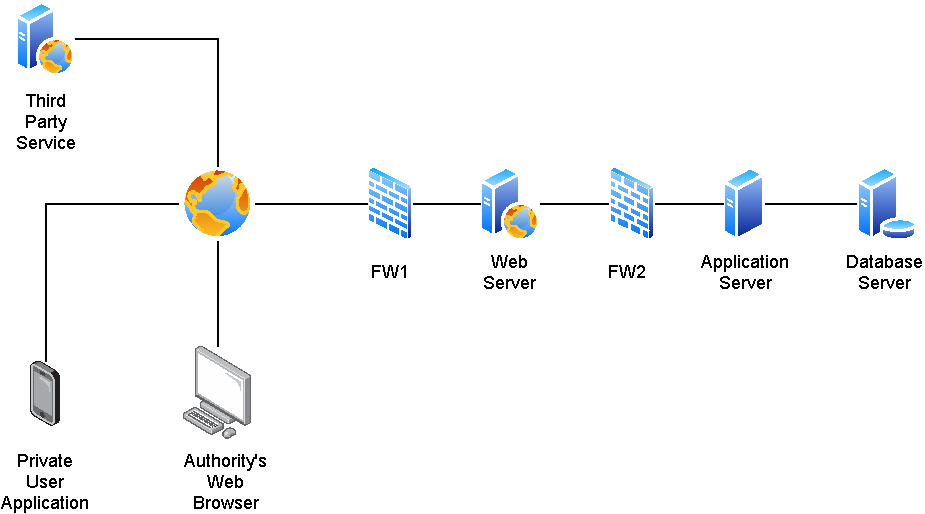
\includegraphics[width=0.9\linewidth]{../assets/sequence_diagrams/exports/architecture.pdf}
		\caption{High Level System Structure}
	\end{figure}
Our system can be summarized into 3 logical layers:
\begin{itemize}
\item \textbf{Presentation Layer}\\
This layer is divided into the Client tier (Mobile App for users) and the Web tier (Web App for authorities). From here, user, authorities and third parties, such as the municipality, can access the system's functionalities and the users' data through the Web Server, protected by a DeMilitarized Zone (DMZ)
\item \textbf{Application Layer}\\
In this layer the application server acts as a set of components accessible to the software developer through a standard API defined for the platform itself. We decided to separate the Application Server from the Web Server mainly for security reasons, and secondly because our application server targets much more than just Web page generation: it implements services like clustering and load-balancing.
\item \textbf{Data Layer}\\
Here we have the Database Server and the Database itself, where all the data about the users, the authorities and the violations reported are stored\\
\end{itemize}
\subsection{Component view}
\subsubsection{High Level Component Diagram}
The following diagrams represents the systems' components and its interfaces throughout which they interact in order to execute their functionalities. We'll divide this view into two sides, the Client side and the Server side:
\begin{itemize}
\item The Client side is composed of three different components, the \texttt{Authority Web Application}, intended for authorities only, the \texttt{Third Party Web Application}, for municipality, and the \texttt{Mobile Application}, for users. The first two refers to the \texttt{AuthoritiesWebServices} service for authorities and to the \texttt{Third Party Web Services} for the municipality, the last to the \texttt{UserMobileServices} service for users
\item The Server side is consequently also composed of three different components, the \texttt{Authorities Web Services} which will enable authorities to check the map, solve violations, etc., the \texttt{User Mobile Services} which gives users the chance to report street/parking violations with pictures, check/modify their personal data and review their report history and the \texttt{Third Party Services}, which is primarily intended for the municipality and enables them to receive and share data-mined information about violations to SafeStreets in order to generate suggested interventions etc.
\end{itemize}
\begin{figure}[H]
		\centering
		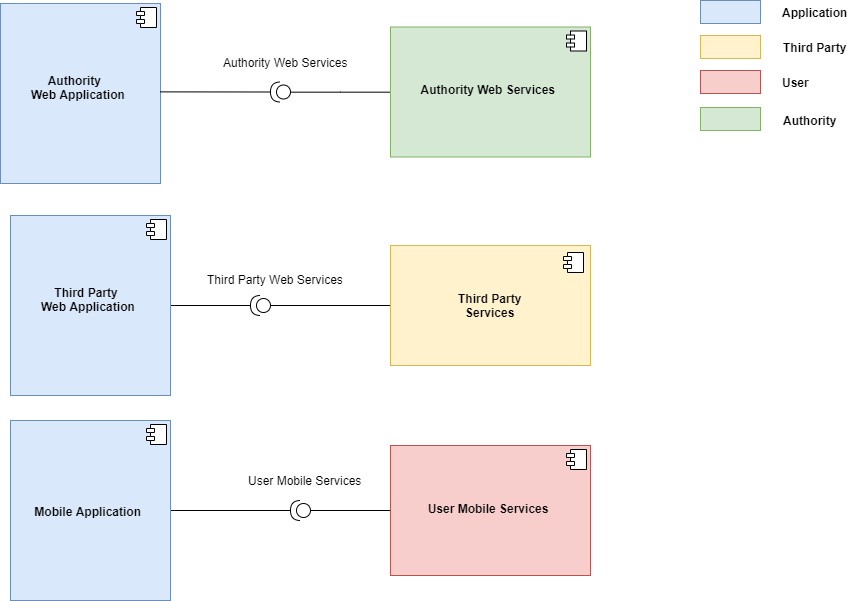
\includegraphics[width=0.9\linewidth]{../assets/images/COMPONENT VIEW.png}
	\end{figure}


\subsubsection{User Mobile Services Projection}
The User Mobile Services Projection is subdivided into 4 modules: the \texttt{Subscription Manager Module}, \texttt{Violation Reporting Module}, the \texttt{Reports History Module} and the \texttt{Profile Manager Module}. These components provide to the User Mobile Application the following interfaces: \texttt{SubscriptionManager}, \texttt{ViolationReport}, \texttt{ReportsHistory} and \texttt{ProfileManager}. These components also need to communicate with a \texttt{SMS Service}, a \texttt{Maps Service}, the \texttt{Camera Service}, the \texttt{ANPR Service} and finally a \texttt{DBMS} which must guarantee full availability and functionality to the Application for a better user experience
\begin{figure}[H]
		\centering
		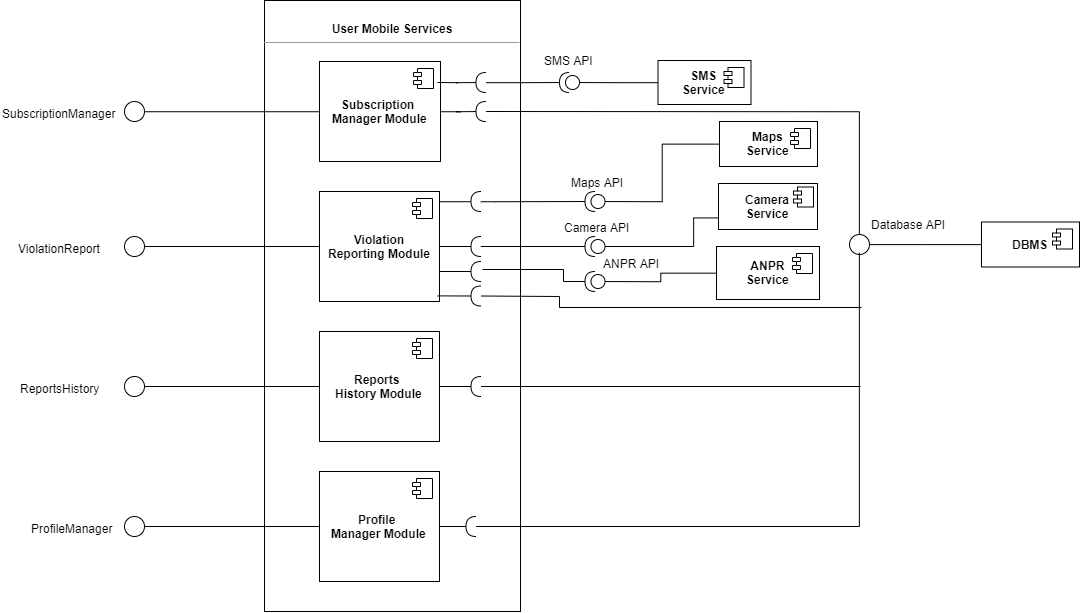
\includegraphics[width=1.2\linewidth]{../assets/images/USER PROJECTION.png}
	\end{figure}
As you can see, every single module have access to the \texttt{DBMS} and the \texttt{Subscription Manager Module} interacts with a \texttt{SMS Service}, where a SMS is sent with a verification code to subscribe to the system. The \texttt{Violation Reporting Module}, the most important in the whole User Mobile Services, interfaces with a \texttt{Maps Service} for the localization of the vehicle, a \texttt{Camera Service} for the acquisition of the vehicles photo and a \texttt{ANPR Service} (Automatic Number Plate Recognition) which recognizes the license plate from the photo and saves it in the Violation Report 
\subsubsection*{Module Functionalities}
\begin{itemize}
\item \textbf{Subscription Manager Module}: this module manages the registration and login processes of the user. It will allow them to insert their personal data and register to the system, and, subsequently, login with the same credentials. 
\item \textbf{Violation Reporting Module}: this module is the most important as it enables the user to report street/parking violations by taking pictures of the vehicle involved and uploading them to the system. 
\item \textbf{Reports History Module}: this module manages the users' report history, and, when requested, queries the data from the database and shows it to the user
\item \textbf{Profile Manager Module}: this module provides all the necessary functions concerning the update and deletion of any existing profile information\\\\
\end{itemize}

\subsubsection{Authority Web Services Projection}
The Authority Web Services Projection is subdivided into 4 modules: the \texttt{Data Access Module}, the \texttt{Authentication Manager Module}, the \texttt{Violation Solving Module} and the \texttt{Suggestion Generating Module}. These components provide to the Authority Web Application the following interfaces: \texttt{Data Access}, \texttt{Authentication Manager}, \texttt{Violation Solving} and \texttt{Suggestion Generating} . These components also need to communicate with a \texttt{PRA Service}, \texttt{Machine Learning Service} and finally a \texttt{DBMS} for the same reasons mentioned above.
\begin{figure}[H]
		\centering
		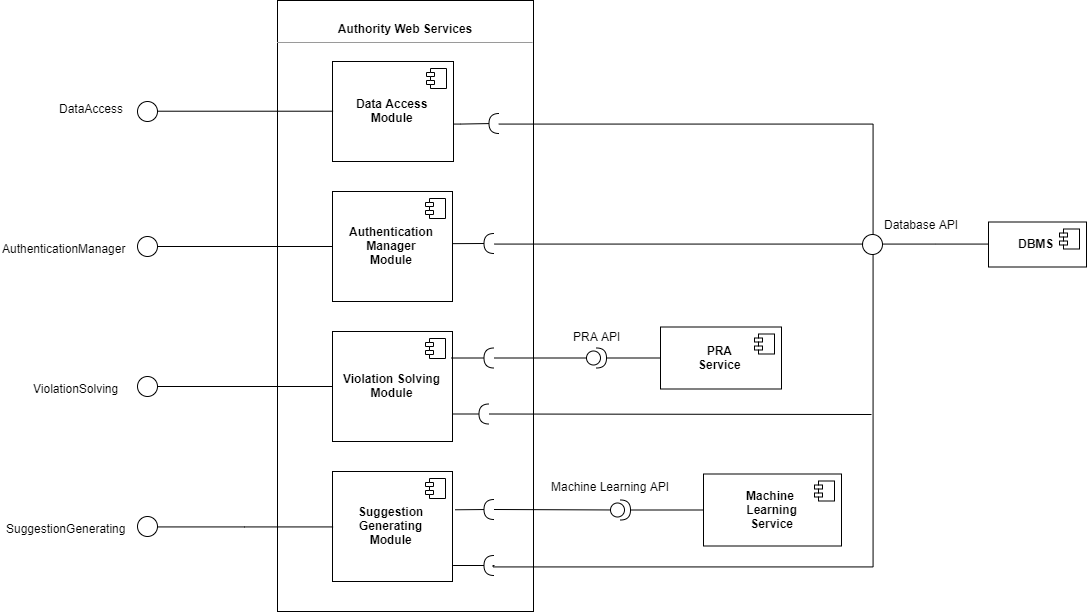
\includegraphics[width=1.2\linewidth]{../assets/images/AUTH PROJECTION.png}
	\end{figure}
We can see here how authorities refer to the PRA (Pubblico Registro Automobilistico) to gather data from the license plates through the \texttt{PRA Service} while the \texttt{Machine Learning Service} is needed in order to generate suggestions for interventions to take in streets particularly full of violations.
\subsubsection*{Module Functionalities}
\begin{itemize}
\item \textbf{Data Access Module}: this module deals with the access to violations reported by users, while no private data is accessed 
\item \textbf{Authentication Manager Module}: this module manages the registration and login of the authority. It will allow them to insert their personal data and to receive their AUC and DBP in order to successfully register to the system.
\item \textbf{Violation Solving Module}: this module lets the authority interact with the list of violations, checking their validity and solving them. 
\item \textbf{Suggestion Generating Module}: this module manages the generation of suggestions on possible interventions to take in order to prevent violations from being committed in that precise area.
\end{itemize}
\newpage
\subsubsection{Third Party Services Projection}
The Third Party Services Projection is subdivided into 2 modules: the \texttt{Data Sharing Module} and the \texttt{Authentication Manager Module}. These components provide to the Third Party Web Application the following interfaces: \texttt{DataSharing} and \texttt{Authentication Manager}. These components won't communicate with any external API, due to the fact that third party's only task (municipality) is to share its data with SafeStreets
\begin{figure}[H]
		\centering
		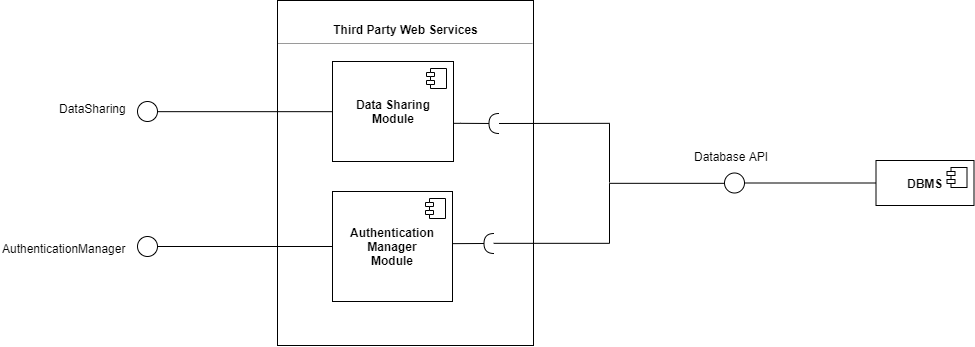
\includegraphics[width=1.2\linewidth]{../assets/images/THIRD PARTY PROJECTION.png}
	\end{figure}
As said above, in our case, the Third Party is intended as the municipality, which have the only task of accessing the software and sharing their data regarding the reports with SafeStreets so when an authority requests it, the software will generate the above mentioned suggestions on interventions.
\subsubsection*{Module Functionalities}
\begin{itemize}
\item \textbf{Data Sharing Module}: this module is in charge of the sharing violation-related mined data to SafeStreets in order to generate suggestions on street interventions to take
\item \textbf{Authentication Manager Module}: this module manages the authentication procedure the municipality must execute to access the Web App
\end{itemize}
\newpage
\subsection{Deployment view}
In order to deploy the system, we decided to implement a 4-tier architecture:
\begin{itemize}
\item \textbf{Tier 1}
The first tier will be composed by the Client (we opted for a Thin Client) that includes a Mobile Application (for users) and a Web Application (for authorities).\\\\
\begin{figure}[H]
		\centering
		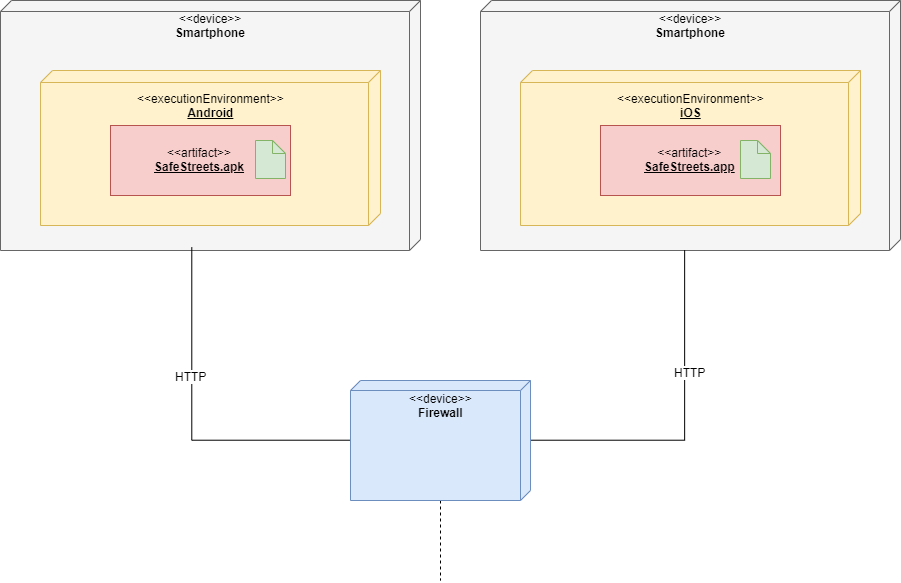
\includegraphics[width=1.0\linewidth]{../assets/images/MOBILE APPLICATION COMP VIEW.png}
		\caption{Tier 1 Deployment View}
	\end{figure}
\newpage
\item \textbf{Tier 2}
This tier corresponds to the Web Server, whose main focus is to store, process static content and deliver web pages to the Clients. Infact, we opted for Apache Tomcat thanks to its high-availability, clustering feature for load balancing and its optimal java-focused environment\\\\
\begin{figure}[H]
		\centering
		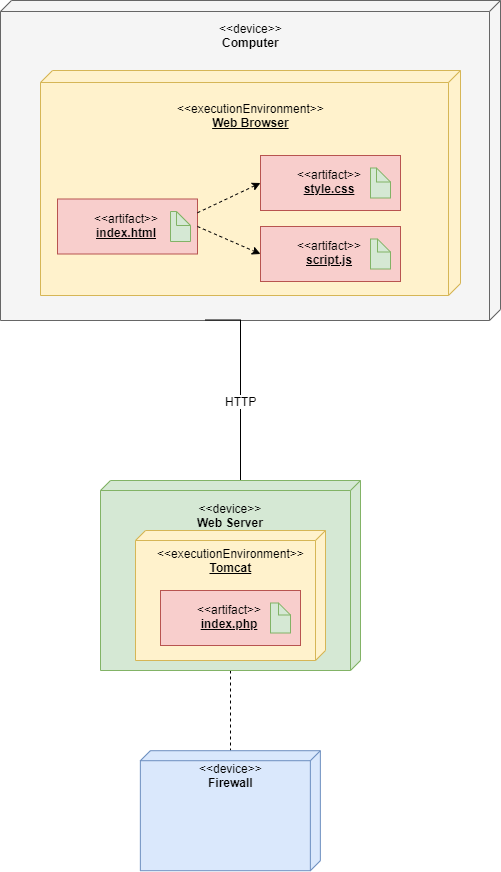
\includegraphics[width=0.5\linewidth]{../assets/images/tier1_tier2.png}
		\caption{Tier 2 Deployment View}
	\end{figure}
\newpage
\item \textbf{Tier 3}
This tier corresponds to the Application Server, that both facilitates the creation of web applications and provides a server environment where to run these applications. We opted for Apache Geronimo, since one of its components is Tomcat, and because of its compatibility with Java EE 6 specifications.\\\\
\begin{figure}[H]
		\centering
		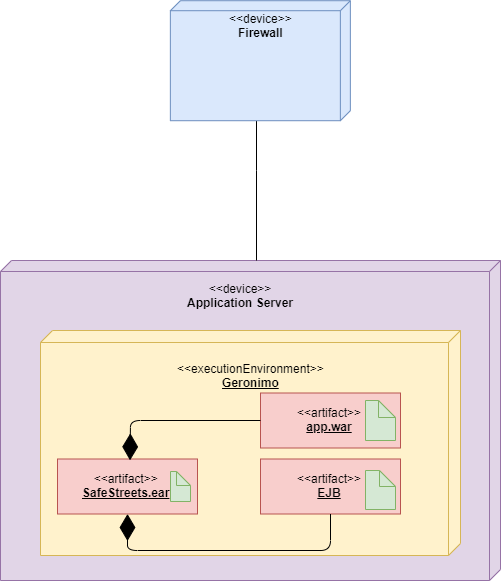
\includegraphics[width=0.5\linewidth]{../assets/images/app_server.png}
		\caption{Tier 3 Deployment View}
	\end{figure}
\newpage
\item \textbf{Tier 4}
The final tier corresponds to the Database Server, where the DBMS is running. We opted for MySQL, since it is one of the most secure and reliable database management system used in popular web applications, while at the same time guarantees scalability and high performance.
\begin{figure}[H]
		\centering
		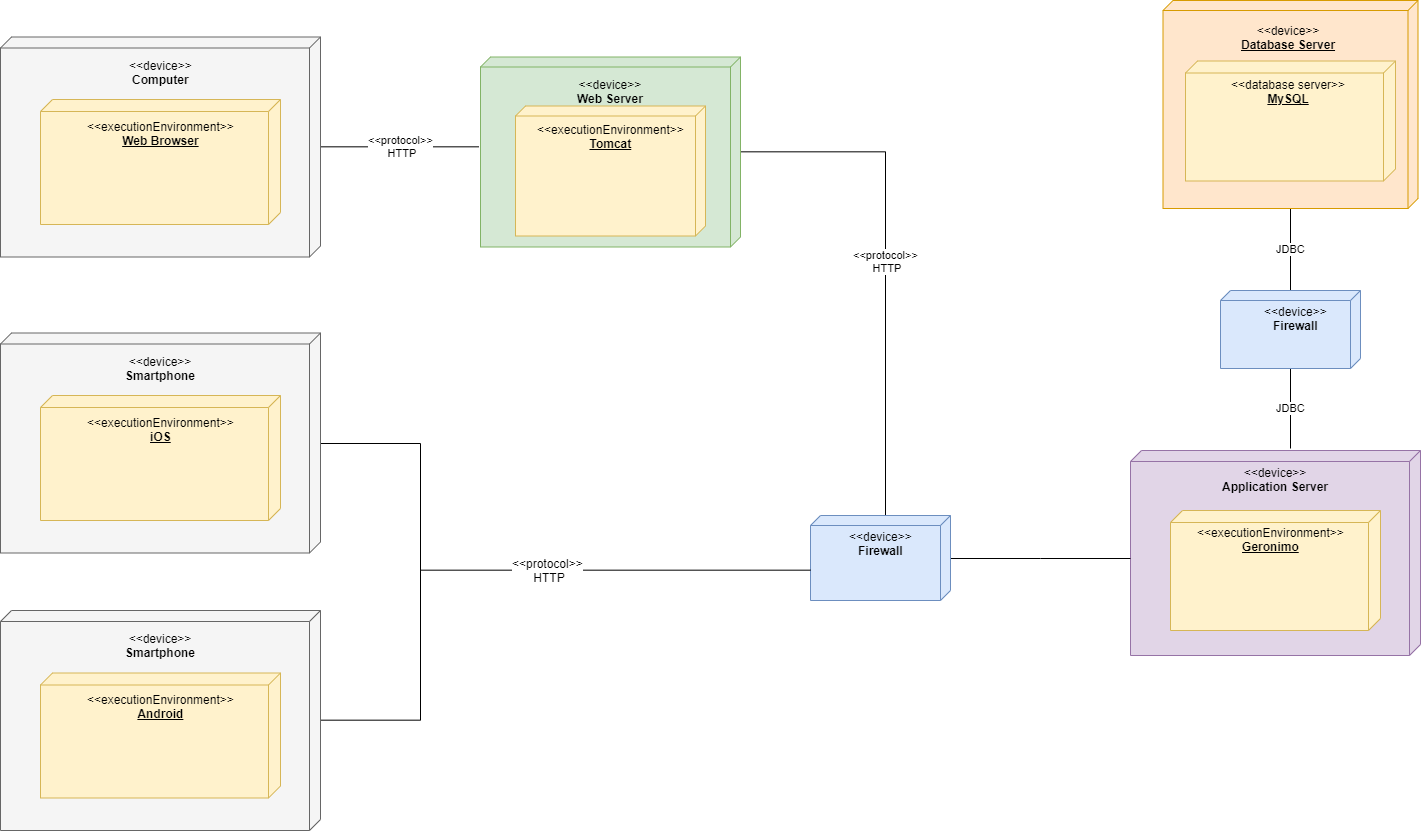
\includegraphics[width=1.0\linewidth]{../assets/images/ENTIRE SYSTEM.png}
		\caption{Entire System Deployment View with Tier 4}
	\end{figure}
\end{itemize}
\subsection{Runtime view}
\subsection{Component interfaces}
\subsubsection{External Interfaces}
SafeStreets uses some Application Programming Interfaces to facilitate the implementation. These components are infact largely used and compatible with most of the devices currently on the market:
\begin{itemize}
\item \texttt{SMS API}: it enables the the possibility to register to the system with a telephone number, thanks to a process in which a temporary code is sent through an SMS Service
\item \texttt{Maps API}: fundamental for the violation reporting functionality, as it shows the user its location and the vehicles location in a well visible map
\item \texttt{Camera API}: every users' smartphone needs direct access to its camera to take pictures of the violation-committing vehicles' license plate
\item \texttt{ANPR API}: Automatic Number Plate Recognition is a technology that uses optical character recognition on images to read vehicle registration plates to create vehicle location data. Its presence in the system is fundamental so the software recognizes the vehicles plate from the photo and saves the data in the database 
\item \texttt{PRA API}: the Pubblico Registro Automobilistico is the big database where any user can infer sensible data regarding a vehicles' owner. In our case, the PRA is accessed by authorities in the process we called Violation Solving where they can take measures towards the vehicles owner
\item \texttt{Machine Learning API}: SafeStreets will use machine learning generate suggestions on interventions to take in streets full of violations. This happens when SafeStreets crosses its own data with the one provided by the municipality when an authority decides to request a suggestion
\item \texttt{Database API}: this API is actually used to support multiple database servers easily, to provide a structured interface for the dynamic construction of queries, to enforce security checks and to facilitate the interaction with the database
\end{itemize}
\newpage
\subsection{Selected architectural styles and patterns}
\subsubsection{Design Patterns}
Here are the design patterns we used to make our architecture more flexible:
\begin{itemize}
\item \textbf{Model View Controller}\\
Nowadays, most Mobile and Web Applications rely on this pattern. These type of applications infact retrieve data from the Database and updates the Users' Interface consequently and according to the provided input, while the Controller checks the validity of the requested operations. Therefore the main scope of this pattern is to separate the Data (Model), the Users' Interface (View) and the user's input validator (Controller)
\begin{figure}[H]
		\centering
		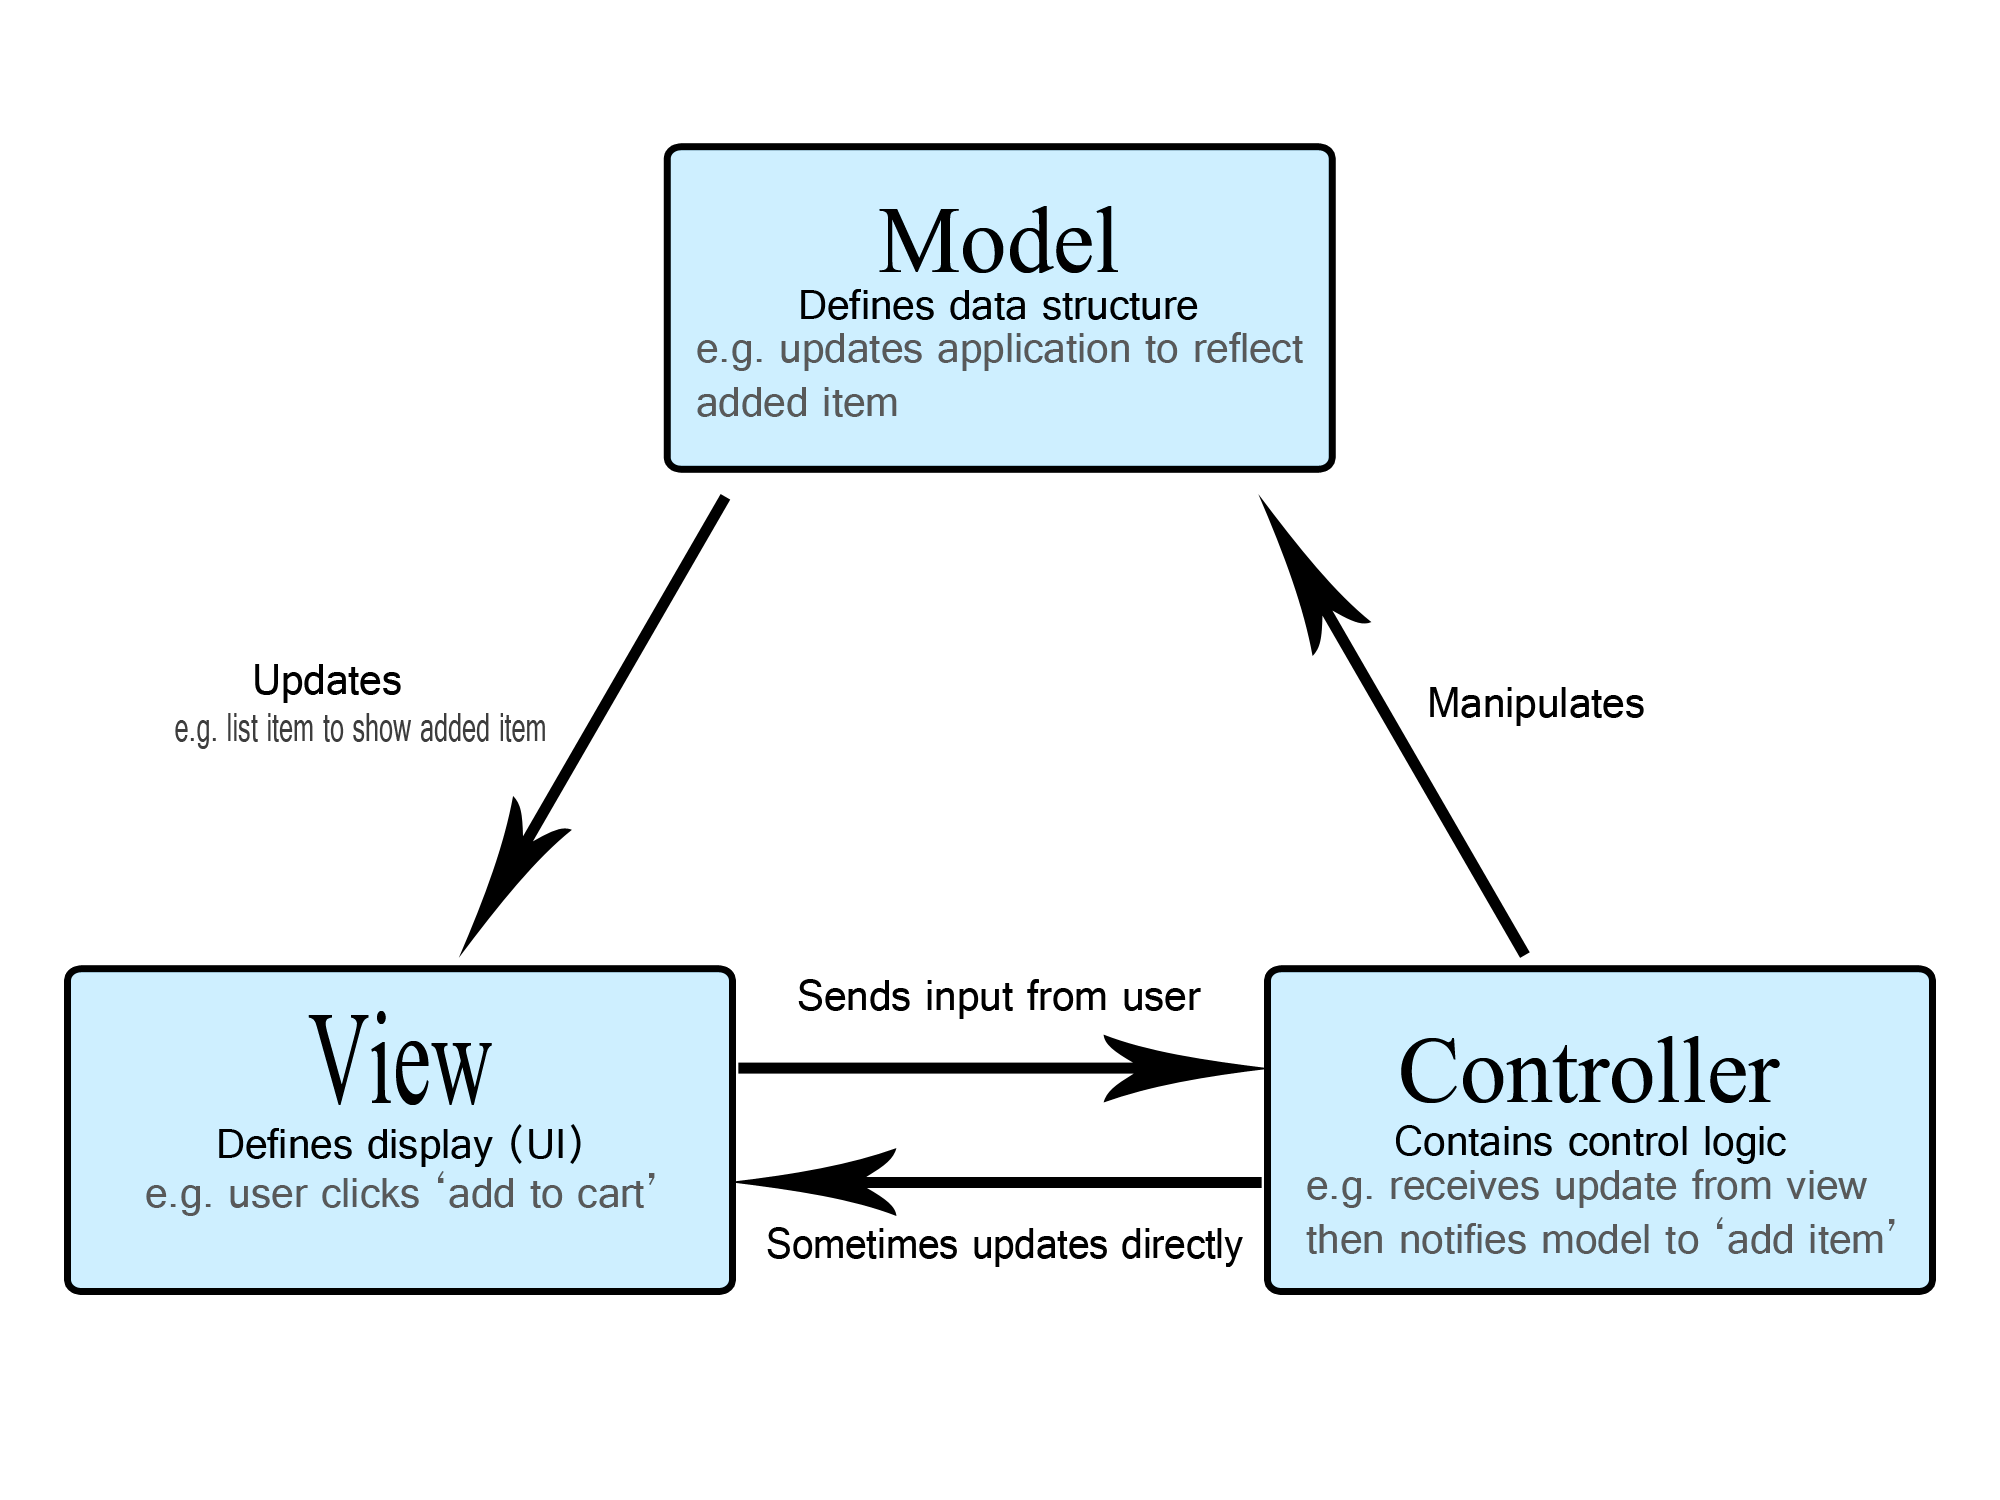
\includegraphics[width=1.0\linewidth]{../assets/images/model-view-controller-light-blue.png}
	\end{figure}
\newpage
\item \textbf{Decorator Pattern}\\
The Decorator is a design pattern that allows behavior to be added to an individual object, dynamically, without affecting the behavior of other objects from the same class. It can be used to extend (decorate) the functionality of a certain object statically, or in some cases at run-time, independently of other instances of the same class, provided some groundwork is done at design time. This is achieved by designing a new Decorator class that wraps the original class. This pattern is designed so that multiple decorators can be stacked on top of each other, each time adding a new functionality to the overridden method. In our case, it can be used to add new information on a already reported violation which lacks in important data without affecting the other violations already compiled
\begin{figure}[H]
		\centering
		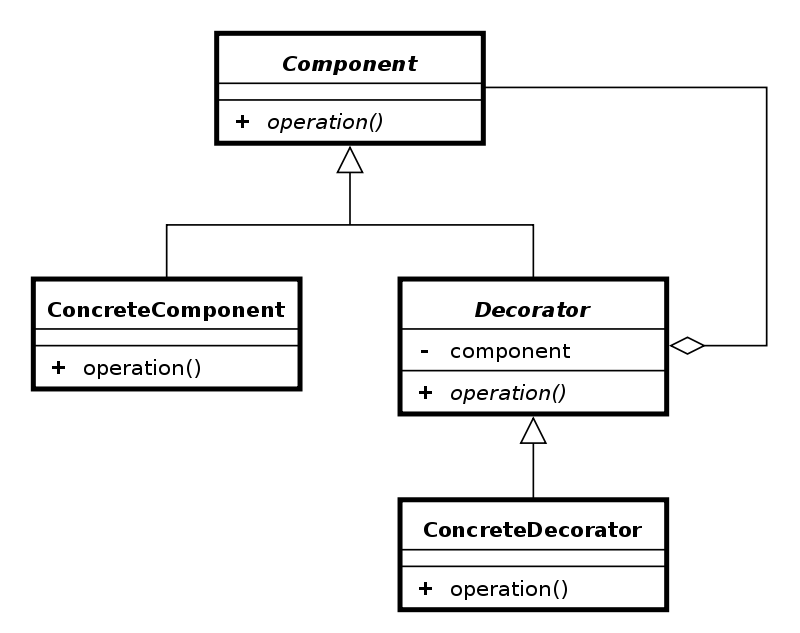
\includegraphics[width=1.0\linewidth]{../assets/images/800px-Decorator_UML_class_diagram.png}
	\end{figure}
\newpage
\item \textbf{Proxy Pattern}\\
It provides a surrogate for another object to control access to it. In our system architecture it can be useful to interface the Application Server with the Database Server. For example, whenever a user, an authority or a third party (municipality) requests some data that is unchanged, the proxy can answer the query without involving access to the database, providing a better response time. In our case, it can be useful when a user requests his reports history or when an authority requests a suggestion
\begin{figure}[H]
		\centering
		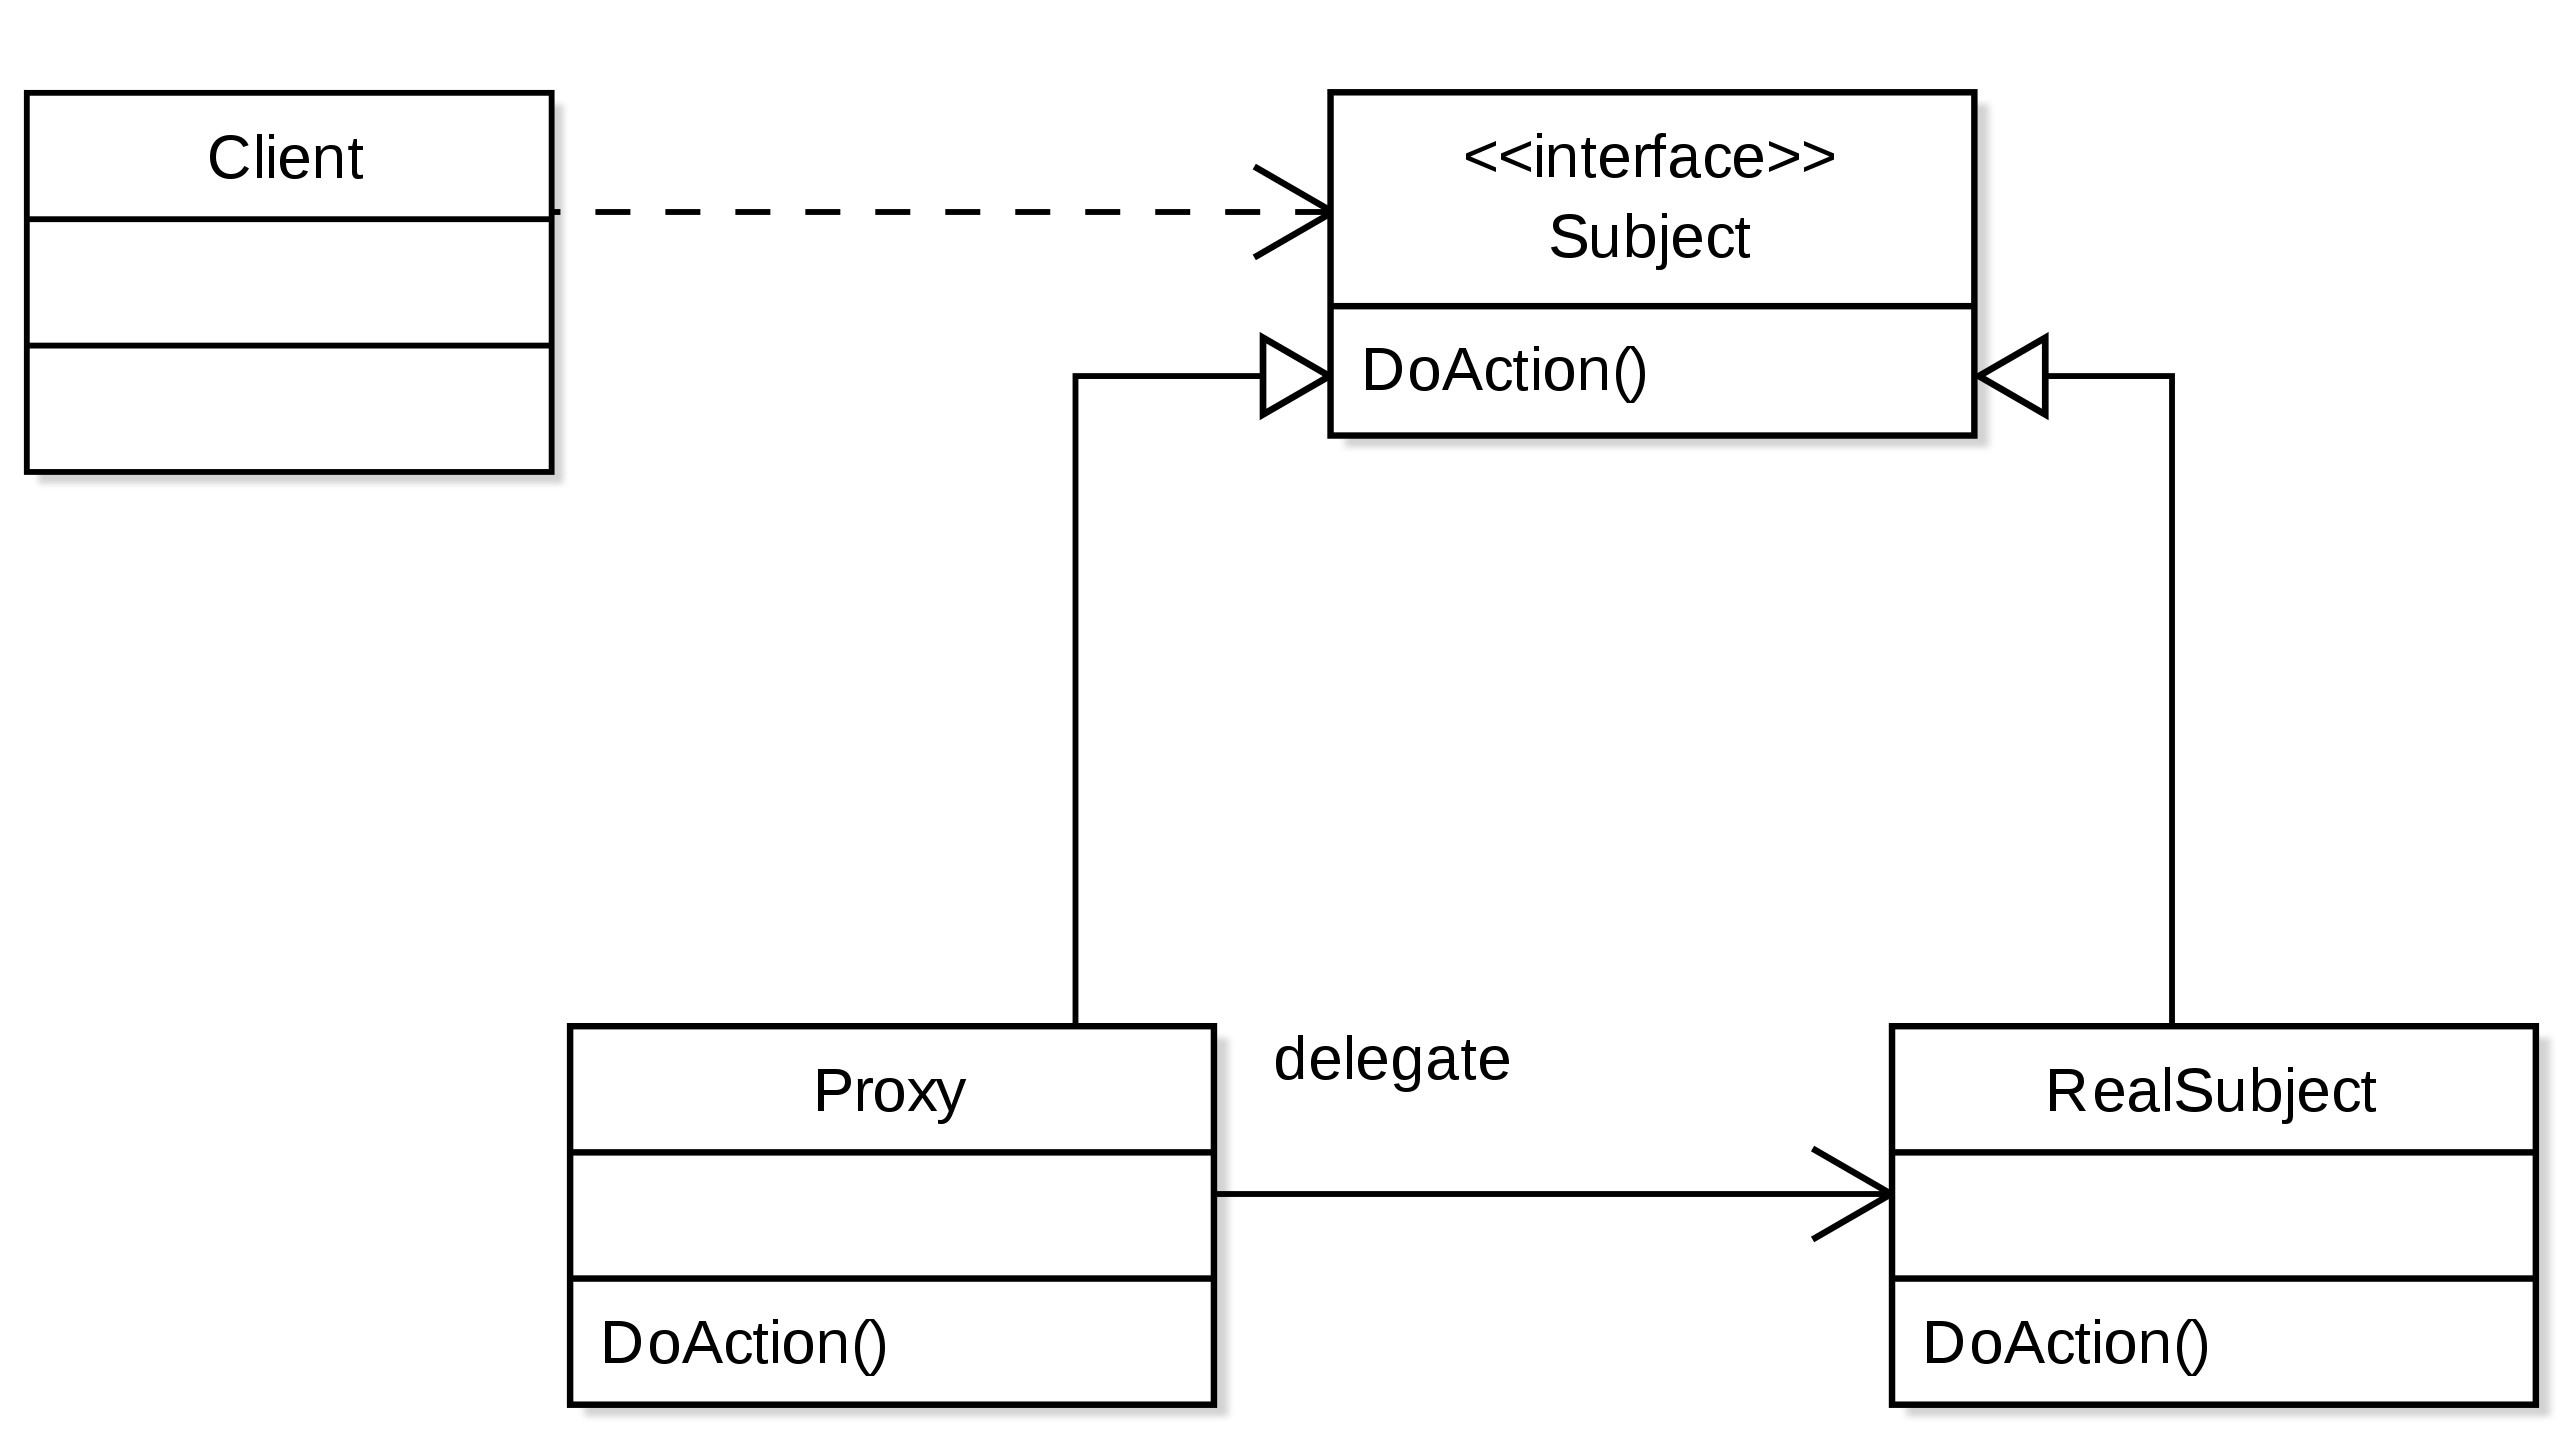
\includegraphics[width=1.0\linewidth]{../assets/images/2560px-Proxy_pattern_diagram.png}
	\end{figure}
\end{itemize}
\subsubsection{RAPS Architecture}
We want our system to rely on a RAPS (Reliable Array of Partitioned Service) architecture, in order to prevent unavailability of some functionalities in case of breakdowns. This architecture consists in a partitioned and redundant structure: servers are cloned to achieve this objective. More precisly, multiple services are divided on different machines and each machine can access in turn to a copy of the stored data. Such architecture guarantees better availability and scalability and provides a high rate of maintainability: in case of breakdowns, it is sufficient to work on the damaged machine, without interfering with the other machines' tasks, while the specific service can still be perfomed. In addition, if the system is willing to expand some services, it is sufficient invest
on the specific partition associated to that service.
\subsection{Other design decisions}

\section{USER INTERFACE DESIGN}
As already mentioned in the \texttt{Requirements Analysis and Specification Document} (RASD), our idea is to provide users with a Mobile App (for smartphones and tablets) and authorities with a Web App (for computers).\\ The applications will be different both in functionalities and in style, and we decided to separate the two and therefore make them exclusive, because of the different use and different authentication method they have.\\ For a closer look at what the two interfaces look like, we invite you to check our RASD where several mock-ups have been presented
\section{REQUIREMENTS TRACEABILITY}
\subsubsection*{[R1]: The system must allow users to provide their credentials and personal data}
\begin{itemize}
\item Components
\begin{itemize}
\item SubscriptionManager
\end{itemize}
\end{itemize}
\subsubsection*{[R2]: The system must let the user verify his account with his e-mail or by SMS}
\begin{itemize}
\item Components
\begin{itemize}
\item SubscriptionManager
\item SMS Service
\end{itemize}
\end{itemize}
\subsubsection*{[R3]: The system must verify there are no other registered users with the same e-mail or telephone number}
\begin{itemize}
\item Components
\begin{itemize}
\item SubscriptionManager
\item DBMS
\end{itemize}
\end{itemize}
\subsubsection*{[R4]: In order to register successfully, the system must oblige the user to accept the data privacy policies and conditions}
\begin{itemize}
\item Components
\begin{itemize}
\item SubscriptionManager
\end{itemize}
\end{itemize}
\subsubsection*{[R5]: The system must give the user the possibility to take pictures}
\begin{itemize}
\item Components
\begin{itemize}
\item ViolationReport
\item Camera Service
\end{itemize}
\end{itemize}
\subsubsection*{[R6]: The system must retrieve the users' position correctly}
\begin{itemize}
\item Components
\begin{itemize}
\item ViolationReport
\item Maps Service
\end{itemize}
\end{itemize}
\subsubsection*{[R7]: The system must recognize the license plate}
\begin{itemize}
\item Components
\begin{itemize}
\item ViolationReport
\item ANPR Service
\end{itemize}
\end{itemize}
\subsubsection*{[R8]: The system must give the user the chance to select a violation type from the dropdown menu}
\begin{itemize}
\item Components
\begin{itemize}
\item ViolationReport
\end{itemize}
\end{itemize}
\subsubsection*{[R9]: The system musn't give the user the possibility to load photos from their device}
\begin{itemize}
\item Components
\begin{itemize}
\item ViolationReport
\item Camera Service
\end{itemize}
\end{itemize}
\subsubsection*{[R10]: If the users' wants to, the system must let them write an optional description.}
\begin{itemize}
\item Components
\begin{itemize}
\item ViolationReport
\end{itemize}
\end{itemize}
\subsubsection*{[R11]: The system must show to the user all the violations he reported in the past}
\begin{itemize}
\item Components
\begin{itemize}
\item ReportsHistory
\end{itemize}
\end{itemize}
\subsubsection*{[R12]: The system must show to the user his account information and personal data when requested}
\begin{itemize}
\item Components
\begin{itemize}
\item ProfileManager
\end{itemize}
\end{itemize}
\subsubsection*{[R13]: The system must allow authorities to provide their credentials and personal authority identification}
\begin{itemize}
\item Components
\begin{itemize}
\item AuthenticationManager
\end{itemize}
\end{itemize}
\subsubsection*{[R14]: The system must verify there are no other registered authorities with the same identification}
\begin{itemize}
\item Components
\begin{itemize}
\item AuthenticationManager
\item DBMS
\end{itemize}
\end{itemize}
\subsubsection*{[R15]: In order to register successfully, the system must oblige the authority to accept the data privacy policies and conditions}
\begin{itemize}
\item Components
\begin{itemize}
\item AuthenticationManager
\end{itemize}
\end{itemize}
\subsubsection*{[R16]: The system must allow authorities to access the Violations Map and see which type of violations are being committed where}
\begin{itemize}
\item Components
\begin{itemize}
\item ViolationSolving
\item DataAccess
\item DBMS
\end{itemize}
\end{itemize}
\subsubsection*{[R17]: The system must allow authorities to switch to the Suggestions Map and see which suggestions have been posted for each area}
\begin{itemize}
\item Components
\begin{itemize}
\item SuggestionGenerating
\item DataAccess
\item DBMS
\end{itemize}
\end{itemize}
\subsubsection*{[R18]: The system must allow authorities to discard pictures which don't represent a vehicle}
\begin{itemize}
\item Components
\begin{itemize}
\item DataAccess
\end{itemize}
\end{itemize}
\subsubsection*{[R19]: The system must allow authorities to discard pictures of vehicles which aren't committing any violation}
\begin{itemize}
\item Components
\begin{itemize}
\item DataAccess
\item ViolationSolving
\end{itemize}
\end{itemize}
\section{IMPLEMENTATION, INTEGRATION AND TEST PLAN}
\section{EFFORT SPENT}	\
\begin{itemize}
		\item Giancarlo Danese
		\begin{center}
			\begin{tabular}{| c | c | c |}
				\hline
				Day & Subject & Hours \\ \hline
				18/11/2019 & Purpose, Scope & 2 \\
				21/11/2019 & Architectural Design & 2\\
				24/11/2019 & Diagrams & 2\\
				27/11/2019 & Diagrams & 2\\
				30/11/2019 & Component View & 2\\
				\hline
			\end{tabular}
		\end{center}

		\item Davide Savoldelli
		\begin{center}
			\begin{tabular}{| c | c | c |}
				\hline
				Day & Subject & Hours \\ \hline
				18/11/2019 & Architectural Design & 1 \\
				24/11/2019 & Diagrams & 2 \\
				27/11/2019 & Diagrams & 2 \\
				30/11/2019 & Deployment View & 2\\
				\hline
			\end{tabular}
		\end{center}
	\end{itemize}
\section{REFERENCES}



\end{document}